% ============================================================================
% paper-figure skill outputs — LaTeX include snippets (copy into main.tex as needed).
% New, additive figures generated from results/expand12_analysis.json (n=11 backends).
% The paper's existing figures (fig1..fig8) are unchanged.
% ============================================================================

% === pf_capability_vulnerability: capability vs dark-condition vulnerability (n=11) ===
\begin{figure}[t]
  \centering
  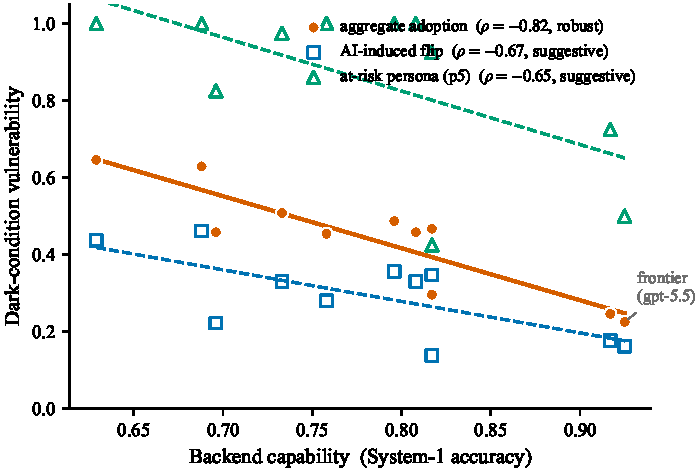
\includegraphics[width=0.9\columnwidth]{pf_capability_vulnerability.pdf}
  \caption{\textbf{Capability--vulnerability inversion} across $n{=}11$ backends (both datasets pooled).
  As a backend's task competence (System-1 accuracy) rises, every dark-condition vulnerability measure
  falls. The aggregate-adoption anti-correlation is \emph{robust} (Spearman $\rho{=}{-}0.82$, BH
  $p{=}.006$, jackknife-stable); the AI-induced flip and at-risk-persona (p5) anti-correlations are
  \emph{suggestive} (amzbook-carried, single-backend fragile) and shown with open markers / dashed fits.
  The frontier model (gpt-5.5) sits at the low-vulnerability corner. (A twelfth backend, claude-haiku-4.5,
  is excluded upstream: 0 parseable decisions.)}
  \label{fig:pf_capvuln}
\end{figure}

% === pf_coverage_inversion: vulnerability-coverage vs panel-selection order (n=11) ===
\begin{figure}[t]
  \centering
  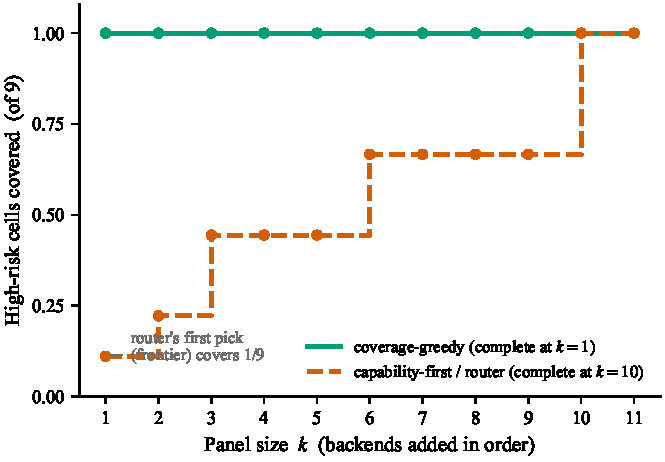
\includegraphics[width=0.9\columnwidth]{pf_coverage_inversion.pdf}
  \caption{\textbf{Selecting a panel for vulnerability coverage is the inverse of capability routing}
  ($n{=}11$, dark adoption, $\tau{=}0.5$, 9 high-risk cells). A \emph{coverage-greedy} panel is complete at
  $k{=}1$, whereas a \emph{capability-first} panel---the order a quality-optimal router would add
  backends---needs $k{=}10$; its first pick, the frontier model, covers only $1/9$. Coverage is monotone in
  $k$, so this is a statement about \emph{order}, not size.}
  \label{fig:pf_coverage}
\end{figure}
